%%%%%%%%%%%%%%%%%%%%%%%%%%%%%%%%%%%%%%%%%%%%%%%%%%%%%%%%%%%%%%%%
%
% Apuntes de la asignatura Modelos Matemáticos I.
% Doble Grado de Informática y Matemáticas.
% Universidad de Granada.
% Curso 2016/17.
% 
% 
% Colaboradores:
% Javier Sáez (@fjsaezm)
% Daniel Pozo (@danipozodg)
% Pedro Bonilla (@pedrobn23)
% Guillermo Galindo
% Antonio Coín (@antcc)
% Sofía Almeida (@SofiaAlmeida)
%
% Agradecimientos:
% Andrés Herrera (@andreshp) y Mario Román (@M42) por
% las plantillas base.
%
% Sitio original:
% https://github.com/libreim/apuntesDGIIM/
%
% Licencia:
% CC BY-NC-SA 4.0 (https://creativecommons.org/licenses/by-nc-sa/4.0/)
%
%%%%%%%%%%%%%%%%%%%%%%%%%%%%%%%%%%%%%%%%%%%%%%%%%%%%%%%%%%%%%%%


%------------------------------------------------------------------------------
%   ACKNOWLEDGMENTS
%------------------------------------------------------------------------------

%%%%%%%%%%%%%%%%%%%%%%%%%%%%%%%%%%%%%%%%%%%%%%%%%%%%%%%%%%%%%%%%%%%%%%%%
% Plantilla básica de Latex en Español.
%
% Autor: Andrés Herrera Poyatos (https://github.com/andreshp) 
%
% Es una plantilla básica para redactar documentos. Utiliza el paquete  fancyhdr para darle un
% estilo moderno pero serio.
%
% La plantilla se encuentra adaptada al español.
%
%%%%%%%%%%%%%%%%%%%%%%%%%%%%%%%%%%%%%%%%%%%%%%%%%%%%%%%%%%%%%%%%%%%%%%%%%

%%%
% Plantilla de Trabajo
% Modificación de una plantilla de Latex de Frits Wenneker para adaptarla 
% al castellano y a las necesidades de escribir informática y matemáticas.
%
% Editada por: Mario Román
%
% License:
% CC BY-NC-SA 3.0 (http://creativecommons.org/licenses/by-nc-sa/3.0/)
%%%

%%%%%%%%%%%%%%%%%%%%%%%%%%%%%%%%%%%%%%%%
% Short Sectioned Assignment
% LaTeX Template
% Version 1.0 (5/5/12)
%
% This template has been downloaded from:
% http://www.LaTeXTemplates.com
%
% Original author:
% Frits Wenneker (http://www.howtotex.com)
%
% License:
% CC BY-NC-SA 3.0 (http://creativecommons.org/licenses/by-nc-sa/3.0/)
%
%%%%%%%%%%%%%%%%%%%%%%%%%%%%%%%%%%%%%%%%%


% Tipo de documento y opciones.
\documentclass[11pt, a4paper, titlepage]{article}


%---------------------------------------------------------------------------
%   PAQUETES
%---------------------------------------------------------------------------

% Idioma y codificación para Español.
\usepackage[utf8]{inputenc}
\usepackage[spanish, es-tabla, es-lcroman, es-noquoting]{babel}
\selectlanguage{spanish} 
%\usepackage[T1]{fontenc}

% Fuente utilizada.
\usepackage{courier}    % Fuente Courier.
\usepackage{microtype}  % Mejora la letra final de cara al lector.

% Diseño de página.
\usepackage{fancyhdr}   % Utilizado para hacer títulos propios.
\usepackage{lastpage}   % Referencia a la última página.
\usepackage{extramarks} % Marcas extras. Utilizado en pie de página y cabecera.
\usepackage[parfill]{parskip}    % Crea una nueva línea entre párrafos.
\usepackage{geometry}            % Geometría de las páginas.

% Símbolos y matemáticas.
\usepackage{amssymb, amsmath, amsthm, amsfonts, amscd}
\usepackage{upgreek}

% Otros.
\usepackage{enumitem}   % Listas mejoradas.
\usepackage[hidelinks]{hyperref}
\usepackage{pgfplots}
\usepackage{graphicx}            % Gráficos.

%---------------------------------------------------------------------------
%   OPCIONES PERSONALIZADAS
%---------------------------------------------------------------------------

% Redefinir letra griega épsilon.
\let\epsilon\upvarepsilon

% Formato de texto.
\linespread{1.1}            % Espaciado entre líneas.
\setlength\parindent{0pt}   % No indentar el texto por defecto.
\setlist{leftmargin=.5in}   % Indentación para las listas.

% Estilo de página.
\pagestyle{fancy}
\fancyhf{}
\geometry{left=3cm,right=3cm,top=3cm,bottom=3cm,headheight=1cm,headsep=0.5cm}   % Márgenes y cabecera.

% Redefinir entorno de demostración (reducir espacio superior)
\makeatletter
\renewenvironment{proof}[1][\proofname] {\vspace{-15pt}\par\pushQED{\qed}\normalfont\topsep6\p@\@plus6\p@\relax\trivlist\item[\hskip\labelsep\it#1\@addpunct{.}]\ignorespaces}{\popQED\endtrivlist\@endpefalse}
\makeatother

% Aumentar el tamaño del interlineado
\linespread{1.3}
%---------------------------------------------------------------------------
%   COMANDOS PERSONALIZADOS
%---------------------------------------------------------------------------

% Valor absoluto: \abs{}
\providecommand{\abs}[1]{\lvert#1\rvert}    

% Fracción grande: \ddfrac{}{}
\newcommand\ddfrac[2]{\frac{\displaystyle #1}{\displaystyle #2}}

% Texto en negrita en modo matemática: \bm{}
\newcommand{\bm}[1]{\boldsymbol{#1}}

% Línea horizontal.
\newcommand{\horrule}[1]{\rule{\linewidth}{#1}}

% Renombrar la R de los reales

\newcommand{\R}{\mathbb{R}}



%---------------------------------------------------------------------------
%   CABECERA Y PIE DE PÁGINA
%---------------------------------------------------------------------------

% Cabecera del documento.
\renewcommand\headrule{
	\begin{minipage}{1\textwidth}
		\hrule width \hsize 
	\end{minipage}
}

% Texto de la cabecera.
\lhead{\subject}  % Izquierda.
\chead{}            % Centro.
\rhead{\docauthor}    % Derecha.

% Pie de página del documento.
\renewcommand\footrule{                                 
	\begin{minipage}{1\textwidth}
		\hrule width \hsize   
	\end{minipage}\par
}

% Texto del pie de página.
\lfoot{}                                                 % Izquierda
\cfoot{}                                                 % Centro.
\rfoot{Página\ \thepage\ de\ \protect\pageref{LastPage}} % Derecha.


%---------------------------------------------------------------------------
%   ENTORNOS PARA MATEMÁTICAS
%---------------------------------------------------------------------------

% Nuevo estilo para definiciones.
\newtheoremstyle{definition-style} % Nombre del estilo.
{10pt}               % Espacio por encima.
{10pt}               % Espacio por debajo.
{}                   % Fuente del cuerpo.
{}                   % Identación.
{\bf}                % Fuente para la cabecera.
{.}                  % Puntuación tras la cabecera.
{.5em}               % Espacio tras la cabecera.
{\thmname{#1}\thmnumber{ #2}\thmnote{ (#3)}}     % Especificación de la cabecera (actual: nombre en negrita).

% Nuevo estilo para notas.
\newtheoremstyle{remark-style} 
{10pt}                
{10pt}                
{}                   
{}                   
{\itshape}          
{.}                  
{.5em}               
{}                  

% Nuevo estilo para teoremas y proposiciones.
\newtheoremstyle{theorem-style}
{10pt}                
{10pt}                
{\itshape}           
{}                  
{\bf}             
{.}                
{.5em}               
{\thmname{#1}\thmnumber{ #2}\thmnote{ (#3)}}                   

% Nuevo estilo para ejemplos.
\newtheoremstyle{example-style}
{10pt}                
{10pt}                
{}                  
{}                   
{\scshape}              
{:}                 
{.5em}               
{}                   

% Teoremas, proposiciones y corolarios.
\theoremstyle{theorem-style}
\newtheorem*{nth}{Teorema}
\newtheorem*{nprop}{Proposición}
\newtheorem{ncor}{Corolario}

% Definiciones.
\theoremstyle{definition-style}
\newtheorem*{ndef}{Definición}

% Notas.
\theoremstyle{remark-style}
\newtheorem*{nota}{Nota}

% Ejemplos.
\theoremstyle{example-style}
\newtheorem*{ejemplo}{Ejemplo}

% Listas ordenadas con números romanos (i), (ii), etc.
\newenvironment{nlist}
{\begin{enumerate}
\renewcommand\labelenumi{(\emph{\roman{enumi})}}}
{\end{enumerate}}

% División por casos con llave a la derecha.
\newenvironment{rcases}
  {\left.\begin{aligned}}
  {\end{aligned}\right\rbrace}

%---------------------------------------------------------------------------
%   PÁGINA DE TÍTULO
%---------------------------------------------------------------------------

% Título del documento.
\newcommand{\subject}{Modelos Matemáticos I}

% Autor del documento.
\newcommand{\docauthor}{Doble Grado de Informática y Matemáticas}

% Título
\title{
  \normalfont \normalsize 
  \textsc{Universidad de Granada} \\ [25pt]    % Texto por encima.
  \horrule{0.5pt} \\[0.4cm] % Línea horizontal fina.
  \huge \subject\\ % Título.
  \horrule{2pt} \\[0.5cm] % Línea horizontal gruesa.
}

% Autor.
\author{\Large{\docauthor}}

% Fecha.
\date{\vspace{-1.5em} \normalsize Curso 2016/17}


%---------------------------------------------------------------------------
%   COMIENZO DEL DOCUMENTO
%---------------------------------------------------------------------------
\begin{document}

\maketitle  % Título.
\tableofcontents    % Índice
\vfill
\begin{center}
\includegraphics{../Recursos/Plantillas/by-nc-sa.eps}  % Licencia.
\end{center}
\newpage


%----------------------------
%   Introducción.
%----------------------------
\section*{Introducción.}
En esta asignatura, intentaremos estudiar una serie de modelos que se dan en la naturaleza y que explican cosas de 




\newpage

\section{Ecuaciones en diferencias de primer orden}

Para motivar este tema, vamos a poner primero unos ejemplos de ecuacinoes en diferencias de primer orden.

\begin{enumerate}
	\item Progresión geométrica, una ecuación de la forma:
\[
x_{n+1} =  \alpha x_n
\]

Para dar una solución, deberíamos establecer el valor de $x_n$ de forma explícita. En este caso, una solución sería:
\[
x_n = \mathcal{C} \alpha^n
\]

Donde $\mathcal{C}$ es una constante. Así, $x_0 = \mathcal{C}$.

\item Progresión aritmética, es decir, una de la forma:
\[
x_{n+1} = x_n + \beta
\]
donde una solución sería:
\[
x_n = \mathcal{C} + n\beta
\]

\item La sucesión de Fibonacci es otro ejemplo de una ecuación en diferencias.

\[
x_{n+2} = x_{n+1} + x_{n}
\]

\end{enumerate}

\begin{ndef}[Ecuación en diferencias]
	Una ecuación en diferencias es una ecuación en la que intervienen un número fijo de términos consecutivos de una sucesión.
	\[
	F(x_{n+k},\dots, x_n , n)= 0
	\]
donde $F$ es una función de varias variables, $\{x_n\}$ es una sucesión, las incógnitas y $k \geq 1 $ es el orden de la ecuación
\end{ndef}

Como ejemplo de cálculo de órdenes, podríamos que decir de la progresión aritmética y geométrica son de orden 1 y la sucesión de Fibonacci es de orden 2.

\begin{ndef}[Resolución de una ecuación en diferencias]
	Resolver una ecuación en diferencias es hallar la forma explícita de todas las sucesiones que satisfacen la igualdad, la solución general. Una solución concreta de la ecuación se llama solución particular y generalmente se obtiene a partir de $k$ condiciones iniciales en la solución general.
\end{ndef}

\begin{nota}
	Una propiedad de las progresiones geométricas es que si la progresión converge, converge a 0. Si no converge, puede ser cíclica, divergente o alternada.
\end{nota}

\begin{ndef}[Ecuación en diferencias lineal]
	Una ecuación en diferencias lineal viene dado por una ecuación de la forma:

\[
a_k(n)x_{n+k} + ... + a_0(n)x_n = b(n)
\]
Si $a_k(n)\ne 0 \ , \ n \geq 0$ se dice que es de orden $k$. Si $b(n) = 0$, se dice que la ecuación es homogénea.
\end{ndef}


\subsection{Ecuación en diferencias de primer orden lineal con coeficientes constantes}

Una ecuación en diferencias de primer orden lineal será de la forma:
\[
x_{n+1} = \alpha x_n +  \beta \quad \alpha,\beta \in \mathbb{C}
\]
Estas ecuaciones serán de orden 1 con coeficientes constantes.

\begin{nprop}
	La solución de estas ecuaciones será:
	\begin{nlist}
	\item Si $\beta = 0$ es una progresión geométrica así que $x_n =  \mathcal{C} \alpha^n$
	\item Si $\beta \ne 0$ y $\alpha  = 1$ entonces es una progresión aritmética, así que $x_n = \mathcal{C} + \beta$
	\item Si $\beta \ne 0 $ y $\alpha \ne 1 $ entonces la ecuación tiene una solución constante:
	\[
	x_* = \frac{\beta}{1-\alpha}
	\]
	Esta solución satisfacerá la ecuación si no dependiera de $n$.
\end{nlist}
\end{nprop}
\begin{proof}
	Probaremos la tercera, que es la que no es trivial.\\
	Buscaremos entonces una solución constante $x_*$. Si es solución, debe verificar que:
$$x_* =  \alpha x_* + \beta \implies  x_* = \dfrac{\beta}{1 - \alpha}$$
\end{proof}

\begin{ejemplo}
	Comprobar si en el caso 3, una solución podría ser: \[x_n = \alpha^n x_0 + \beta \sum_{i=0}^{n-1}\alpha^i\]
\end{ejemplo}

\begin{nprop}
	Si $\alpha \ne 1$, la sucesión $\{x_n\}$ es solución de la ecuación $\iff$ la sucesión $\{z_n\}$ definida por $z_n = x_n - x_*$ es solución de la ecuación:
	\[
	z_{n+1} =  \alpha z_n
	\]
\end{nprop}
\begin{proof}
	Si $\{x_n\}_{n\geq 0}$ es solución de (1) $\implies \bar{x}_{n+1}= \alpha\bar{x}_n+\beta$
	
	
	Además, $\{x_*\}$ es solución de (1) $\implies \bar{x}_{*}= \alpha\bar{x}_*+\beta$
	
	Ahora, restamos ambas y nos queda:
	\[
	\bar{x}_{n+1} - \bar{x}_*= \alpha (\bar{x}_n - \bar{x}_*).
	\]
	Por lo que hemos obtenido una solución de la ecuación (2), pues si $\bar{z}_n= \bar{x}_n - \bar{x}_*\implies \bar{z}_{n+1}= \alpha \bar{z}_n \implies \{\bar{z}_n\}_{}$
	
\end{proof}






\begin{ejemplo}
	Resuelva $x_{n+1} = -ix_n + 3$. Esto es una ecuación en diferencias de primer orden lineal no homogénea.
	\begin{proof}[Solución]
	Primero, calculamos la solución constante: $x_n = x_*$ para $n \geq 0$. Esta es:
	\[
	x_* = -i x_* +3 \implies x_* = \frac{3}{1+i}
	\]
	
	Calculamos ahora la ecuación homogénea asociada, esta es $z_{n+1} = -iz_n$ con $n \geq 0$. Así, $z_n =  \mathcal{C}(-i)^n$.
	
	Ahora, una solución de la ecuación inicial sería:
	\[
	x_n =  x_* +z_n = \frac{3}{1+i}+\mathcal{C}(-i)^n
	\]
\end{proof}

\end{ejemplo}

\begin{nprop}
	Si $\alpha \ne 1$, la ecuación:
	\[
	x_{n+1} = \alpha x_n + \beta
	\]
	entonces la ecuación tiene tantas soluciones como valores posibles tenga la condición inicial:
	\[
	x_n = x_* + (x_0-x_*)\alpha^n , \ \ \ n=0,1,2...
	\]
	
	\begin{proof}
	Si $x_{n+1} = \alpha x_n + \beta$ y $\alpha \ne 1$, las soluciones de son de la forma:
	\[
	x_n = x_*+z_n 
	\]
	con $z_n$ una solución homogénea asociada y $x_*$ una solución constante.
	\[
	z_{n+1} = \alpha z_n \implies z_{n} = \mathcal{C}\alpha^n \implies z_n = (x_o - x_*)\alpha^n \implies x_n = x_o + (x_0 - x_*)\alpha^n
	\]
	
\end{proof}

\end{nprop}


\begin{ejemplo}
	$x_{n+1}=ix_n+1 \ \ n \geq 0$ con $x_0=i$
	\begin{proof}[Solución]
	Primero hallamos la solución constante:
	\[
	x_* = \frac{1}{1-i} \implies x_* = ix_* +1
	\]
	Ahora, hallamos la solución homogénea asociada:
	\[
	z_{n+1} = iz_n \text{con $z_n = \mathcal{C}i^n$}
	\]
	Seguidamente, hallamos la solución de la ecuación completa:
	\[
	x_n = x_* + z_n = \frac{1}{1-i}+ \mathcal{C}i^n
	\]
	
	Por último, aplicamos la condición inicial $x_0=i$ dada. Así:
	\[
	x_0 = \frac{1}{1-i}+ \mathcal{C}i \implies \mathcal{C} = i-\frac{1}{1-i} =  \frac{i+1-1}{1-i} = \frac{i}{1-i} = \frac{i(1+i)}{2} = \frac{-1}{2}+ \frac{1}{2}i
	\]
	De esta forma, la solución sería:
	\[
	x_n = \frac{1}{1-i} + (\frac{-1}{2}+ \frac{1}{2}i)i^n
	\]
	Y esto se podría pasar a forma estándar de número complejo.
\end{proof}
\end{ejemplo}

\begin{ejemplo}[2]
	$x_{n+1}=(3-2i)x_n -1$ para $n\geq 0$. 
	\begin{proof}[Solución]
	Tenemos que:
	\[
	x_n = \frac{-1}{1-(3-2i)}+\mathcal{C}(3-2i)^n = \frac{1}{4} + \frac{1}{4}i + \mathcal{C}(3-2i)^n
	\]
\end{proof}
\end{ejemplo}

\begin{nprop}[Fórmula de Moivre]
	Si $\alpha$ es un número complejo, entonces:
	\[
	\alpha^n = r^n(cos(n\theta) + i sin(n\theta))
	\]
	\begin{proof}
	Vamos a hacer un razonamiento por inducción:
	\begin{enumerate}
	\item Si $n=1$. Entonces, $\alpha = r(cos\theta +i\sen\theta)$, trivial.
	\item Supuesto cierto para cierto $n$, lo demostraremos para $n+1$:
	\[
	\alpha^{n+1} = \alpha\alpha^n =  [r(cos(\theta) +i\sen(\theta))] [r^n(cos(n\theta) +i\sen(n\theta))]=
	\]
	\[
	r^{n+1}[cos(\theta) cos(n\theta) +i sen(\theta) cos(n\theta) + isen(n\theta) cos(\theta) - sen(\theta) sen(n\theta)] = \]
	\[r^{n+1}[cos(\theta+n\theta)+isen(\theta+n\theta)] = r^{n+1}[cos((n+1)\theta)+isen((n+1)\theta)]
	\]
\end{enumerate}
	
\end{proof}
\end{nprop}

\begin{nota}
	Esto es porque un número complejo es de la forma $\alpha = a+bi$ = $r(cos\theta + i sin\theta)$.
	Donde el módulo es $r=\sqrt{a^2 + b^2}$ y $\theta$ es el ángulo, tal que $0 \leq \theta \leq 2\pi$.
	$(cos\theta + i sin\theta)$ tiene módulo 1.
	
\end{nota}

\subsection{Comportamiento asintótico de las soluciones}
Tendríamos en este caso que estudiar cómo se comporta la sucesión $\{\alpha^n\}$ con $\alpha \in \mathbb{C}$.
\begin{nprop}\hfill
\begin{nlist}
	\item $|\alpha|< 1 \implies \{\alpha^n\}\to 0$
	\item $|\alpha|> 1 \implies \{|\alpha|^n\}\to +\infty$
	\item $|\alpha| = 1 \implies \alpha^n \in \mathbb{S}^1$
\end{nlist}
	
\end{nprop}

Ahora, si tuviéramos una ecuación de la forma:
\[
x_{n+1}= \alpha x_n + \beta
\]
Ya sabemos que su solución sería:
\[
x_* +z_n = x_* + \mathcal{C}\alpha^n
\]
Por tanto tendríamos que estudiar cómo varía $\alpha^n$.


\begin{nth}[Comportamiento asintótico de las soluciones]
	Las soluciones $\{x_n\}_{n\geq0}$ de la ecuación:
\[
x_{n+1} = \alpha x_n + \beta
\]

verifican:

\begin{itemize}
\item Si $|\alpha| < 1$, se tiene que ${x_n} \to x_*$
\item Si $|\alpha| > 1$, se tiene que ${x_n}$ diverge.
\item Si $|\alpha| = 1$, entonces ${x_n}$ oscila alrededor de $x_*$, esto es, $x_n$ está en la circunferencia de centro $x_*$ y radio $|x_0 - x_*|$.
\end{itemize}\vspace{0.5cm}

	\begin{proof}
	Si tenemos que:
	\[
x_{n+1}= \alpha x_n + \beta
\]
Ya sabemos que su solución sería:
\[
x_* +z_n = x_* + \mathcal{C}\alpha^n
\]. Entonces:
\begin{nlist}
	\item $|\alpha|< 1 \implies \{\alpha^n\}\to 0 \implies \{x_n\} \to x_*$
	\item $|\alpha|> 1 \implies \{|\alpha|^n\}\to +\infty \implies \{|x_n|\}$ nos da el mismo comportamiento que $|\alpha|^n$
	\item $|\alpha| = 1 \implies \alpha^n \in \mathbb{S}^1$ si tomamos módulos y despejamos, tenemos que:
	\[
	|x_n -x_*| = |G|
	\]
	Así que todas las soluciones se mantienen en la circunferencia de centro $x_*$ y radio $|x_0-x_*|$
\end{nlist}
\end{proof}
\end{nth}

\section{Modelo de la telaraña}
En este modelo, tendremos dos funciones con las que trabajaremos. 
\begin{itemize}
	\item Una función oferta, $O(p)$ que depende del precio $p$
	\item Una función demanda, $D(p)$, que también depende del precio $p$
\end{itemize}

Supondremos ahora que estas dos funciones son rectas, para simplificar el sistema. Por ello, tendremos:
\begin{itemize}
\item $O(p) = a+bp $ con $b>0$ la marginal de la oferta
\item $D(p) = c -dp $ con $d> 0$ la marginal de la demanda
	
\end{itemize}
Sin embargo, estas funciones tienen que ajustarse haciendo una estimación con los datos anteriores. Se supone que habrá un punto de equilibrio entre la oferta y la demanda, lo que será un punto de corte entre estas dos funciones establecidas. A este punto lo llamaremos $p_*$. Igualando las ecuaciones, tendríamos que:
\[
 (b+d)p_*= c-a \implies p_* = \frac{c-a}{b+d}
\]

Ahora, para que este precio sea correcto, tenemos que tener que b y d sean mayores que cero para no dividir por cero, y que el precio sea positivo, así que supondremos que $c> a$.

Ahora, para trabajar con esa antelación, lo que intentamos hacer es que:
\[
D(p_n) = O(p_{n-1)} \implies c-dp_n = a+bp_{n-1}
\]
Lo cual es una ecuación en diferencias de primer orden, que se puede seguir despejando como:
\[
p_{n+1} = \dfrac{-b}{d}p_n+ \dfrac{c-a}{d}
\]

Y ahora, resolvemos:
\[
p_n = x_* + z_n = p_* + \mathcal{C}(\frac{-b}{d})^n
\] tenemos que 
\[
x_* = \frac{\beta}{1-\alpha} = \frac{(c-a)/d}{(1-(-b/d)}= \frac{c-a}{b+d} = p_*
\]
Por tanto, tenemos que conseguir que $p_n \to p_*$ y para ello tenemos que conseguir que, como $p_{n+1} =p_* + \mathcal{C}(\frac{-b}{d})^n$, entonces tenemos que hacer que $|\dfrac{-b}{d}| < 1 \implies b < d$.
Por ello, lo que tenemos en las rectas es que la pendiente (b) de la recta de la oferta sea menor que la pendiente de la demanda (d).

\section{El model de Verhulst}

Primero, estudiaremos un primer acercamiento que hubo a este modelo

\subsection{La ecuación de Malthus}
Vamos a estudiar ahora una ecuación que modeliza la evolución de la población de una determinada especie en un hábitat sin limitación de alimentos. Esta primera suposición ya no es real, pues siempre hay limitaciones.

Vamos a llamar:
\begin{itemize}
	\item $P_n$ es el número de individuos en el periodo de tiempo $n$. $P_n\geq 0 $
	\item $\alpha_n$ es la tasa de fertilidad o natalidad por individuo. $\alpha_n \in \R^+$
	
	De esta forma, $\alpha_n P_n$ será el número de nacimientos en el periodo n.
	\item $\alpha_m$ es la tasa de mortalidad. $0 < \alpha_m < 1$, pues esta es un tanto por ciento y tenemos que:
	
	Así, $\alpha_m P_n$ será el número de muertes en el periodo n.
\end{itemize}

Una vez presentadas las incógnitas, podemos afirmar que la población en el siguiente periodo será:
\[
P_{n+1} = P_n + \alpha_n P_n - \alpha_m P_n \implies P_{n+1}=(1+\alpha_m-\alpha_m)P_n
\]
Esto es una ecuación en diferencias lineal de primer orden homogénea. En realidad, es una progresión geométrica y por tanto una solución es:
\[
P_n =\mathcal{C} (1+\alpha_n-\alpha_m)^n \ \ n \geq 0
\]
Pero esta constante es la población inicial, luego eso es equivalente a:
\[
P_n =P_0 (1+\alpha_n-\alpha_m)^n \ \ n \geq 0
\]
Vamos a llamar entonces a $(1+\alpha_n-\alpha_m) = R$ la razón de crecimiento.
\begin{itemize}
	\item $(1+\alpha_n-\alpha_m) > 1 \implies \{P_n\}\to +\infty$. Ahora, esto ocurrirá si y sólamente si $\alpha_n > \alpha_m$
	
	\item $(1+\alpha_n-\alpha_m) < 1 \implies \{P_n\}\to 0$. Del mismo modo, esto sólo ocurre si $\alpha_n < \alpha_m$
	
	\item $(1+\alpha_n-\alpha_m) = 1 \implies \{P_n\} \to P_0$. Que ocurre si y solo si $\alpha_n = \alpha_m$.
\end{itemize}

Se cumple siempre que $R = \dfrac{P_{n+1}}{P_n}$.

\begin{ndef}[Razón de crecimiento]
	Llamaremos razón de crecimiento a:
	\[
	\alpha = \alpha_n - \alpha_m
	\]
	Que representa la variación del tamaño de la población por individuo. Además, podemos ver despejando de la ecuación inicial que:
	\[
	\alpha = \dfrac{P_{n+1}-P_n}{P_n}
	\]
	
\end{ndef}

\subsection{El modelo de Verhulst}
Esto quiso dar un arreglo a la ecuación de Malthus. Ahora, suponemos que en el hábitat hay un número máximo de individuos al que llamaremos $M$.

Según Verhulst, la tasa de crecimiento es proporcional a $M-P_n$, esto es:
\[
\alpha = \dfrac{P_{n+1}-P_n}{P_n} = K (M-P_N) \quad K > 0
\]

De aquí, podemos ver fácilmente que si $P_n < M \implies P_{n+1} > P_n$, por lo que la población crece.

También, si $P_n > M \implies P_{n+1} < P_n$, por lo que la población decrece.

Por tanto, con el modelo de Verhulst desarrollando en la euación de Malthus la ecuación será:
\[
P_{n+1} = [(1+K(M-P_n)]P_n \implies P_{n+1} = (1+KM)P_n -KP_n^2
\]
Donde $KP_n^2$ lo llamaremos la \textbf{competencia entre individuos}.

Esto es una ecuación en diferencias \textbf{no lineal} de primer orden y no homogénea. Aún no hemos explicado cómo se resuelven este tipo de ecuaciones, abordaremos este tema más adelante.

Sin embargo, podemos hacer a la ecuación un cambio de variable haciendo que:
\begin{itemize}
	\item $(1+KM) = \mu$
	\item $x_n = \dfrac{K}{1+Km}P_n$
\end{itemize} 
Y nos queda que:
\[
\dfrac{K}{1+Km}P_{n+1} = \dfrac{K}{1+Km}(1+KM)P_n ( 1 - \dfrac{K}{1+Km}P_n)
\]
Y con los términos anteriores esto nos queda como:
\[
x_{n+1} = \mu x_n(1-x_n)
\]
Esta ecuación es conocida como la \textbf{Ecuación Logística}.

\section{Sistemas dinámicos discretos}

\begin{ndef}
	Un sistema dinámico discreto es la descripción formal de un fenómeno evolutivo en términos de una función cuya imagen está contenida en su dominio. Partiendo desde cualquier valor inicial admisible generaremos una sucesión de valores mediante la aplicación reiterada de la función dada. Lo notaremos SDD.
\end{ndef}

\begin{ndef}
	Supongamos que $I \subset \R$ es un intervalo que contiene al menos dos puntos y $f:I \to I$ es una función continua. Entonces, al par $\{I,f\}$ se le llama un SDD de primer orden, autónomo y en forma normal. A $f$ se le llama función de evolución.
\end{ndef}

Con estas definiciones, podemos ver que si $x_0 \in I$ es un valor inicial, podemos generar:
\[
x_1 = f(x_0); \ x_2 = f(x_1) = f(f(x_0)); \ x_3 = f(x_2) = f(f(f(x_0))); \cdots
\]

Estos valores están bién definidoes pues $f(I) \subset I$ y la sucesión así definida es solución de la ecuación en diferencias:
\[
x_{n+1} = f(x_n) \quad n \geq 0
\]
\begin{ejemplo}
	Tomemos $f(x) = cos(x)$, que es continua. Ahora, tenemos que tomar $I \subset \R$ tal que $f(I) \subset I$. Podemos tomar el intervali $I=[-1,1]$ en radianes por supuesto.
	Si tomamos $X_0\in I$, podemos ver fácilmente que $x_{n+1}=f(x_n) \in I$, por lo que $\{[-1,1],cos(x)\}$ es un SDD.
\end{ejemplo}

\begin{nprop}La ecuación logística es un SDD, pues $f(x) = \mu x(1-x)$ es continua y $\exists I = [0,1]: f(I) \subset I$
	
\end{nprop}

\begin{ejemplo}
	Tenemos $f(x) = \dfrac{1}{2}x$, con $I = [0,1]$, $x_{n+1} = \dfrac{1}{2}x_n$. Esta función es continua (en particular es contractiva). $\{[0,1],f\}$ es un SDD.
\end{ejemplo}
\begin{ejemplo}
	$f(x) = log(x)$, $I=(0,+\infty)$ no es un SDD pues $Im(f) \nsubseteq Dom(f)$
\end{ejemplo}

\begin{ndef}
	UN SDD $\{I,f\}$ se dice lineal si $f$ es lineal, afín si $f$ es afín y no lineal si $f$ no es lineal ni afín.
\end{ndef}

Notación. En lo sucesivo, para denotar las sucesivas iteradas de $f$ usaremos que $f^n = f \circ f \circ f \cdots \circ f$


\begin{ndef}[Órbita]
	Dado un SDD $\{I,f\}$ y un $x_0\in I$, la sucesión definida por:
	\[
	\{x_0,\cdots, x_n , \cdots\} = \{x_0,f(x_0),f^2(x_0),\cdots, f^n(x_0), \cdots\}
	\]
	se denomina órbita o trayectoria del SDD $\{I,f\}$ asociada al valor inicial $x_0$ y se denota por $\gamma(I,f,x_0)$
\end{ndef}

\begin{ndef}
	Al conjunto de todas las órbitas asociadas al SDD $\{I,f\}$  a todos los $x_0 \in I$ se le llama retrato de fase.
\end{ndef}

\begin{ndef}[Punto de equilibrio]
	Un número $\alpha \in \R$ se dice que es un punto de equilibrio del SDD $\{I,f\}$ si:
	\[
	\alpha = f(\alpha) \ \ \ \alpha \in I
	\]
	Si tomamos como valor inicial un punto de equilibrio del SDD $x_0 = \alpha$ entonces la órbita resultante es constante y se denomina órbita estacionaria:
	\[
	\gamma(I,f,\alpha) = \{\alpha, \alpha, \cdots\}
	\]
\end{ndef}
\begin{ejemplo}
	Determine los puntos de equilibrio de la ecuación logística:
	\[
	x_{n+1} = \mu x_n(1-x_n)
	\]
	Aquí, $f(x) = \mu x(1-x)$, por lo que
	 \[
	\alpha = f(x) \implies \alpha = \mu \alpha (1-\alpha) \implies \alpha - \mu \alpha(1-\alpha) \implies \alpha[1-\mu(1-\alpha)]
	\]
	Por lo que las soluciones pueden ser:
	\[
	\begin{cases}
	\alpha_1 = 0\\
	1-\mu(1-\alpha) = 0 \xrightarrow{(1)} \alpha_2 = \dfrac{\mu -1}{\mu}
\end{cases}
	\]
	Donde en (1) hemos despejado $\alpha$. Es claro que $\alpha_1 \in [0,1]$. Ahora, ¿$\alpha_2=  \dfrac{\mu -1}{\mu} \in [0,1] $?
	
	% REVISAR ESTILO 
	% ---------------------------------------------
	Obtenemos dos puntos de equilibrio:

	$ \alpha_{1} = 0 \in [0,1] $

	$ \alpha_{2}= \frac{\mu - 1}{\mu} $ ? $\in$ ? $ [0,1] $

	Tenemos que:

	$ 0 \leq \frac{\mu - 1}{\mu} \leq 1 $

	Multiplicando por $\mu$ (podemos porque $\mu > 0$):

	$ 0 \leq \mu - 1 \leq \mu \Leftrightarrow -\mu \leq -1 \leq 0 \Leftrightarrow \mu \geq 1 \geq 0 $

	Luego obtenemos que:

	Si $\mu \geq 1 \Rightarrow \alpha_{2} \in [0,1] $
	%-----------------------------------------------
	%GRÁFICAS (?)
\end{ejemplo}
\end{document}
